\documentclass[tikz,border=2pt]{standalone}
\renewcommand{\familydefault}{\sfdefault}
\usetikzlibrary{arrows.meta,calc,positioning}
\tikzset{every picture/.style={line width=1pt, >=Stealth},
         hl/.style={fill=black, fill opacity=0.12, text opacity=1}}
\begin{document}
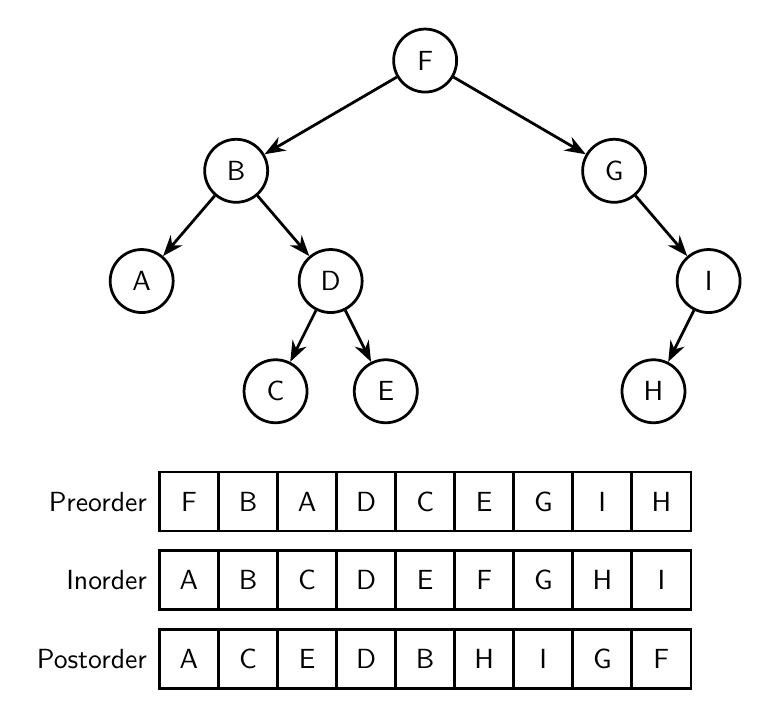
\begin{tikzpicture}[tn/.style={draw, circle, minimum size=0.8cm, inner sep=0pt},
    cell/.style={draw, minimum size=0.75cm}]
  % The same binary tree is used for every traversal on this page.
  \foreach \n/\x/\y in {F/0/0, B/-2.4/-1.4, G/2.4/-1.4, A/-3.6/-2.8, D/-1.2/-2.8, I/3.6/-2.8, C/-1.9/-4.2, E/-0.5/-4.2, H/2.9/-4.2}
    \node[tn] (\n) at (\x, \y) {\n};
  \foreach \a/\b in {F/B, F/G, B/A, B/D, D/C, D/E, G/I, I/H} \draw[->] (\a) -- (\b);

  % \order{y}{name}{nodes}: the order in which a traversal visits the nodes
  \newcommand{\order}[3]{
    \node[anchor=east] at (-3.4, #1) {#2};
    \foreach \v [count=\i from 0] in {#3} \node[cell] at (-3 + 0.75*\i, #1) {\v};
  }
  \order{-5.6}{Preorder}{F, B, A, D, C, E, G, I, H}
  \order{-6.6}{Inorder}{A, B, C, D, E, F, G, H, I}
  \order{-7.6}{Postorder}{A, C, E, D, B, H, I, G, F}
\end{tikzpicture}
\end{document}
